\hypertarget{bonjour-monde}{%
\section{Bonjour, monde !}\label{bonjour-monde}}

\emph{Mardi 24 avril 2018}

Bonjour à tous !

Nous avons le plaisir de dévoiler au monde notre blog, destiné à
héberger les souvenirs à venir de notre voyage. Décollage prévu : 3 mai
2018.

\begin{figure}
\centering
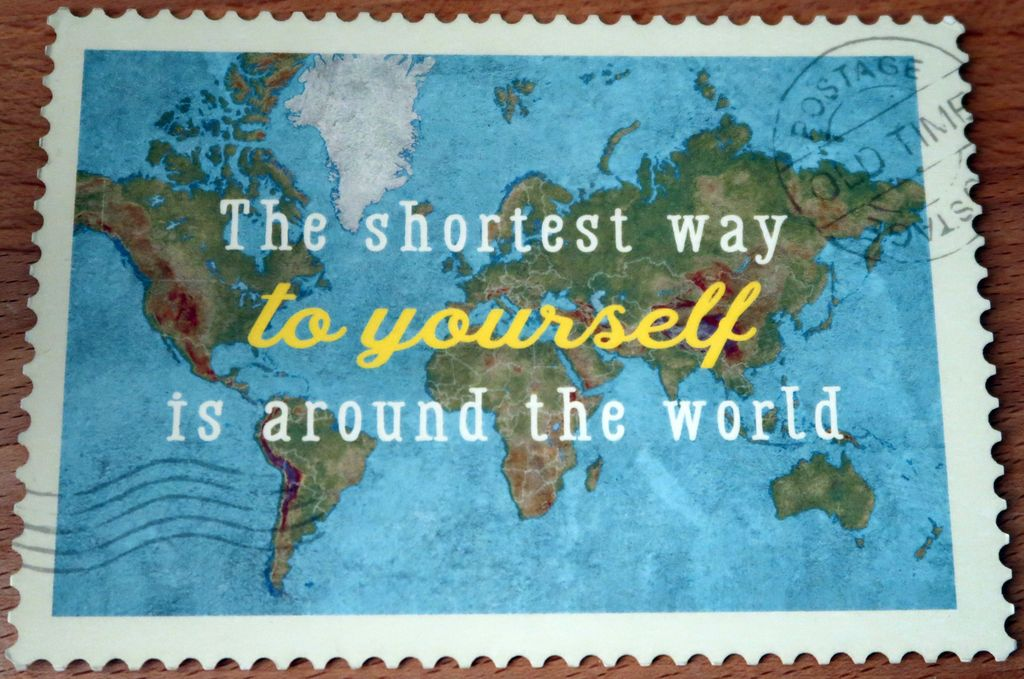
\includegraphics{images/world_postcard.jpg}
\caption{Merci à Marie-Christine pour cette carte postale qui incarne à
merveille l'esprit du voyage...}
\end{figure}

D'ici là, on vous laisse avec deux belles citations avant d'entamer
notre voyage à travers l'espace et à travers le temps :

\begin{quote}
Nous n'aurons de cesse d'explorer et la fin de toutes nos explorations
sera de revenir à l'endroit d'où nous sommes partis et de connaître le
lieu pour la première fois.
\end{quote}

\emph{T. S. Eliot,
\href{https://www.franceinter.fr/emissions/sur-les-epaules-de-darwin/sur-les-epaules-de-darwin-21-avril-2018}{cité
par Jean Claude Ameisen}}

\begin{quote}
"Vous avez longtemps voyagé", dit le Simurgh à ses sujets les oiseaux,
lorsqu'ils le découvrent enfin après une très longue quête, "vous avez
cru parfois vous perdre, mais vous ne vous êtes pas quittés. C'est vous
que vous avez retrouvés."
\end{quote}

\emph{\href{https://fr.wikipedia.org/wiki/La_Conférence_des_oiseaux}{Mantiq
at-Tayr} (La conférence des oiseaux), Farid Al-Din Attar,
\href{https://www.franceinter.fr/emissions/sur-les-epaules-de-darwin/sur-les-epaules-de-darwin-21-avril-2018}{cité
par Jean Claude Ameisen}}

\emph{Elida et Florian}
